\documentclass[a4paper,12pt]{extarticle}
\usepackage[utf8x]{inputenc}
\usepackage[T1,T2A]{fontenc}
\usepackage[russian]{babel}
\usepackage[hidelinks]{hyperref}
\usepackage{indentfirst}
\usepackage{listings}
\usepackage{color}
\usepackage{here}
\usepackage{array}
\usepackage{multirow}
\usepackage{graphicx}
\usepackage{subcaption} 
\usepackage{mathtools}
\usepackage{listings}

\usepackage{caption}
\renewcommand{\lstlistingname}{Программа} % заголовок листингов кода

\bibliographystyle{ugost2008ls}

\usepackage{listings}
\lstset{ %
extendedchars=\true,
keepspaces=true,
language=C,						% choose the language of the code
basicstyle=\footnotesize,		% the size of the fonts that are used for the code
numbers=left,					% where to put the line-numbers
numberstyle=\footnotesize,		% the size of the fonts that are used for the line-numbers
stepnumber=1,					% the step between two line-numbers. If it is 1 each line will be numbered
numbersep=5pt,					% how far the line-numbers are from the code
backgroundcolor=\color{white},	% choose the background color. You must add \usepackage{color}
showspaces=false				% show spaces adding particular underscores
showstringspaces=false,			% underline spaces within strings
showtabs=false,					% show tabs within strings adding particular underscores
frame=single,           		% adds a frame around the code
tabsize=2,						% sets default tabsize to 2 spaces
captionpos=t,					% sets the caption-position to top
breaklines=true,				% sets automatic line breaking
breakatwhitespace=false,		% sets if automatic breaks should only happen at whitespace
escapeinside={\%*}{*)},			% if you want to add a comment within your code
postbreak=\raisebox{0ex}[0ex][0ex]{\ensuremath{\color{red}\hookrightarrow\space}},
texcl=true,
inputpath=listings,                     % директория с листингами
}

\usepackage[left=2cm,right=2cm,
top=2cm,bottom=2cm,bindingoffset=0cm]{geometry}

%% Нумерация картинок по секциям
\usepackage{chngcntr}
\counterwithin{figure}{section}
\counterwithin{table}{section}

%%Точки нумерации заголовков
\usepackage{titlesec}
\titlelabel{\thetitle.\quad}
\usepackage[dotinlabels]{titletoc}

%% Оформления подписи рисунка
\addto\captionsrussian{\renewcommand{\figurename}{Рисунок}}
\captionsetup[figure]{labelsep = period}

%% Подпись таблицы
%\DeclareCaptionFormat{hfillstart}{\hfill#1#2#3\par}
%\captionsetup[table]{format=hfillstart,labelsep=newline,justification=centering,skip=-10pt,textfont=bf}

%% Путь к каталогу с рисунками
\graphicspath{{fig/}}

%% Внесение titlepage в учёт счётчика страниц
\makeatletter
\renewenvironment{titlepage} {
 \thispagestyle{empty}
}
\makeatother

\DeclarePairedDelimiter\abs{\lvert}{\rvert}%
\DeclarePairedDelimiter\norm{\lVert}{\rVert}%

\usepackage{amsmath}

\begin{document}	% начало документа

% Титульная страница
\begin{titlepage}	% начало титульной страницы

	\begin{center}		% выравнивание по центру

		\large Санкт-Петербургский политехнический университет Петра Великого\\
		\large Институт прикладной математики и механики \\
		\large Кафедра <<Прикладная математика>>\\[6cm]
		% название института, затем отступ 6см
		
		%\huge Математическая статистика\\[0.5cm] % название работы, затем отступ 0,5см
		\huge Методы оптимизации\\[0.5cm] % название работы, затем отступ 0,5см
		%\large \textbf{Отчет по лабораторной работе №4}\\[5.1cm]
		\large \textbf{Отчет по лабораторной работе \\``Решение задач одномерной минимизации ``}\\[5.1cm]
		%\\[5cm]

	\end{center}


	\begin{flushright} % выравнивание по правому краю
		\begin{minipage}{0.25\textwidth} % врезка в половину ширины текста
			\begin{flushleft} % выровнять её содержимое по левому краю

				\large\textbf{Работу выполнил:}\\
				\large Колесник В.Н.\\
				\large {Группа:} 3630102/70201\\
				
				\large \textbf{Преподаватель:}\\
				\large к.ф.-м.н., доцент\\
				%\large Баженов Александр Николаевич
				\large Родионова Елена Александровна

			\end{flushleft}
		\end{minipage}
	\end{flushright}
	
	\vfill % заполнить всё доступное ниже пространство

	\begin{center}
	\large Санкт-Петербург\\
	\large \the\year % вывести дату
	\end{center} % закончить выравнивание по центру

\end{titlepage} % конец титульной страницы

\vfill % заполнить всё доступное ниже пространство


% Содержание
\renewcommand\contentsname{\centerline{Содержание}}
\tableofcontents
\newpage

\section{Постановка задачи}
Дана функция:
\begin{equation}
f(x) = 3x+y+4\sqrt{1+x^2+3y^2}
\end{equation}
Заданы точности:
\begin{equation}
\varepsilon_1 = 0.1; \varepsilon_2 = 0.01; \varepsilon_3 = 0.001
\end{equation}
Необходимо найти минимум функции градиентными методами 1-го и 2-го порядка (метод наискорейшего спуска и метод Ньютона) с заданной точностью.\\
Кроме того необходимо проверить ортогональность векторов $x_k-x_{k-1}$ и $x_{k+1}-x_k$ в методе наискорейшего спуска и сравнить два метода.

\section{Исследование применимости методов}
\subsection{Градиентный метод 1-го порядка наискорейшего спуска}
Для доказательства применимости градиентного метода наискорейшего спуска для данной функции воспользуемся следующей теоремой:
\begin{gather}
f(x)\in C^1 \\
\nabla f(x): ||\nabla f(x_1) - \nabla f(x_2)||\leq L ||x_1-x_2||, \forall x_1, x_2 \in R^n \\
\alpha_k: f(x_k-\alpha_k\nabla f(x_k))=\min_{\alpha \in [0,1]} f(x_k-\alpha \nabla f(x_k)) \\
x_k: x_{k+1}=x_k-\alpha_k \nabla f(x_k)
\end{gather}
Тогда $||\nabla f(x_k)||\rightarrow 0$ при $k \rightarrow \infty$ для любого начального приближения $x_0$.\\
\\
Проверим выполнение условия Липшица. Для этого найдем константу $L$ из неравенства, взяв первую норму. Получим:
\begin{gather}
\nonumber||\nabla f(x) - \nabla f(y)||=4|\frac{x_1}{\sqrt{1+x_1^2+3y_1^2}}-\frac{x_2}{\sqrt{1+x_2^2+3y_2^2}}|+\\
\nonumber+12|\frac{y_1}{\sqrt{1+x_1^2+3y_1^2}}-\frac{y_2}{\sqrt{1+x_2^2+3y_2^2}}|\leq L(|x_1-x_2|+|y_1-y_2|)\\
\nonumber\sqrt{1+x_2^2+3y_2^2}\geq 1
\end{gather}
В общем случае найти константу $L$ не удалось. Из неравенства, представленного выше, можно предположить, что $L=12$, так как 12 - наибольшая константа вне модулей. Проверим это предположение численно. Для этого будем генерировать выборку пар двумерных векторов в заданной области и находить максимальное значение следующего отношения по всей выборке:
\begin{equation}
d=\frac{||\nabla f(x_1) - \nabla f(x_2)||}{||x_1-x_2||}
\end{equation}
Для удобства область будет иметь вид:
\begin{equation}
D: -a\leq x \leq a; -b \leq y \leq b.
\end{equation}
Размер выборки был $n=1000$.
В итоге получилось, что для большой области ($a,b>1$) максимальное значение отношения оказалось невелико: $d_{max}\approx 2$. Однако при уменьшении области ($a,b\rightarrow 0$) эта величина стала возрастать. Тем не менее, больше 12 она никогда не становилась ($d_{max}\approx 11.99$).\\
Таким образом, константу Липшица  достаточно взять $L=12$. Условия теоремы выполнены, следовательно метод будет сходиться к решению.

\subsection{Метод Ньютона}
Для доказательства применимости метода Ньютона для данной функции воспользуемся следующей теоремой:
\begin{gather}
f(x)\in C^2 \\
x_2^TH(x_1)x_2: m||x_2||^2\leq x_2^TH(x_1)x_2 \leq M||x_2||^2, \forall x_1, x_2 \in R^n, 0<m<M \\
\alpha_k: f(x_{k+1})-f(x_k)\leq \epsilon\alpha_k \nabla^Tf(x_k)d_k \\
x_k: x_{k+1}=x_k+\alpha_k d_k
\end{gather}
Тогда $x_k\rightarrow x_\ast$ при $k \rightarrow \infty$ для любого начального приближения $x_0$ с квадратичной скоростью.\\
Аналогично предыдущему пункту попробуем получить величины $M, m$ численно.\\ Получим, что константа $M$ увеличивается при уменьшении области $D$, но никогда не превышает 12. Поэтому возьмем $M=12$. \\
При увеличении области $D$ константа $m$ стремится к нулю справа. Возьмем область $D: a=b=5$, в которой находится предполагаемый минимум и в которой будут находиться все $x_k$. Численно получим $m\approx0.01$. Для надежности возьмем $m=0.001$.\\
Таким образом, условия теоремы выполнены, следовательно метод будет сходиться.


\section{Описание алгоритмов}
\subsection{Градиентный метод 1-го порядка наискорейшего спуска}
\subsubsection{Алгоритм}
Пусть задано начальное приближение $x_0$. Положим $k=0$.
\begin{enumerate}
  \item Вычислим $\nabla f(x_k)$
  \item Найдем $\alpha_k=\min_{\alpha \in [0,1]} f(x_k-\alpha \nabla f(x_k))$ методом одномерной минимизации
  \item Положим $x_{k+1}=x_k-\alpha_k \nabla f(x_k)$
  \item Если $||\nabla f(x_{k+1})||^2 < \varepsilon$, то закончим алгоритм с ответом $x_{k+1}$.\\
  Иначе положим $k:=k+1$ и вернемся к шагу 1. 
\end{enumerate}

\subsubsection{Комментарии к алгоритму}
Для получения $\alpha_k$ применялся метод Фибоначчи с той же точностью, что задана для градиентного метода. $\alpha_k$ бралась в середине полученного интервала неопределенности.

\subsection{Метод Ньютона}
\subsubsection{Алгоритм}
Пусть задано начальное приближение $x_0$. Положим $k=0$, $\epsilon=0.25$.
\begin{enumerate}
  \item Вычислим $d_k=-(H(x_k))^{-1}\nabla f(x_k)$
  \item $a_k=1$
  \item Пока не выполнено $f(x_k+\alpha_k d_k)-f(x_k) \leq \epsilon \alpha_k \nabla^T f(x_k)d_k$, пересчитываем $\alpha_k:=\frac{\alpha_k}{2}$
  \item Положим $x_{k+1}=x_k+\alpha_k d_k$
  \item Если $||\nabla f(x_{k+1})||^2 < \varepsilon$, то закончим алгоритм с ответом $x_{k+1}$.\\
  Иначе положим $k':=k+1$ и вернемся к шагу 1. 
\end{enumerate}

\subsubsection{Комментарии к алгоритму}
Обратную матрицу получали следующим образом:
\[A=
\begin{bmatrix}
    a & b\\
    c & d\\
\end{bmatrix}
\]\\
\[A^{-1}=\frac{1}{det A}
\begin{bmatrix}
    d & -b\\
    -c & a\\
\end{bmatrix}
\]

\section{Результаты решения}
Исходная функция достигает минимум в точке:
\begin{equation}
(x, y) = (-\frac{3}{2}\sqrt{\frac{3}{5}}, -\frac{1}{2\sqrt{15}})\approx(-1.1619, -0.1291) 
\end{equation}
В таблице представлены ответы, которые методы дали при заданной точности, и норма разности с реальным ответом. Начальное приближение во всех случаях равно: $x_0=(1,1)$
\begin{table}[h]
	\centering
		\begin{tabular} {|c|c|c|c|c|}
			\hline
			$\varepsilon$ & Гр. м. 1-го порядка & Норма разности & Гр. м. 2-го порядка & Норма разности \\ \hline
			0.1 & $(-0.98,-0.11)$ & 0.18 & $(-1.00,-0.98)$ & 0.16\\ \hline
			0.01 & $(-1.106,-0.117)$ & 0.05 & $(-1.143,-0.126)$ & 0.019\\ \hline
			0.001 & $(-1.1456,-0.1252)$ & 0.016 & $(-1.1430,-0.1260)$ & 0.019\\ \hline
		\end{tabular}
		\caption{Результаты}
	\end{table}
	
\section{Дополнительные исследования}
\subsubsection{Сравнение методов}
Количество вычислений функции, градиента и матрицы Гессе представлено в таблице.
\begin{table}[h]
	\centering
		\begin{tabular} {|c|c|c|c|c|c|c|}
			\hline
			 & \multicolumn{3}{|c|}{Гр. м. 1-го порядка} & \multicolumn{3}{|c|}{Гр. м. 2-го порядка}\\
			\hline
			$\varepsilon$ & $f(x)$ & $\nabla f(x)$ &$H(x)$ & $f(x)$ & $\nabla f(x)$ &$H(x)$  \\ \hline
			0.1 & 30 &6 & 0 & 12 & 4 & 3\\ \hline
			0.01 & 110 &11 & 0 & 14 & 5 & 4\\ \hline
			0.001 & 224 & 15 & 0 & 14 & 5 & 4\\ \hline
		\end{tabular}
		\caption{Количество обращений}
	\end{table}

Из таблицы видно, что для градиентного метода наискорейшего спуска повышение заданной точности в 10 раз приводит к возрастанию в разы количества обращений к целевой функции. Для метода Ньютона аналогичное увеличение точности приводит к увеличению количества обращений ко всем 3 функциям (сама функция, градиент, Гессиан) всего лишь на 1-3 обращения.\\
Это значит, что метод Ньютона эффективнее метода наискорейшего спуска с точки зрения объемов обращений к функциям. Более того, он сходится намного быстрее (4-5 итераций против 6-15). Однако, для его работы требуется Гессиан, который не нужен в методе 1-го порядка.

\subsubsection{Ортогональность векторов в методе наискорейшего спуска}
В таблице представлены наибольшие по модулю значения скалярных произведений нормированных векторов $x_k-x_{k-1}$ и $x_{k+1}-x_k$ для заданных точностей, полученных во время работы метода наискорейшего спуска. Также приведены графики хода метода.

\begin{table}[h]
	\centering
		\begin{tabular} {|c|c|}
			\hline
			$\varepsilon$ & $max(p_k, p_{k-1})$\\ \hline
			0.1 & 0.2513\\ \hline
			0.01 & 0.0179 \\ \hline
			0.001 & 0.0038\\ \hline
		\end{tabular}
		\caption{Скалярные произведения}
	\end{table}

\begin{figure}[!htb]
    \centering
    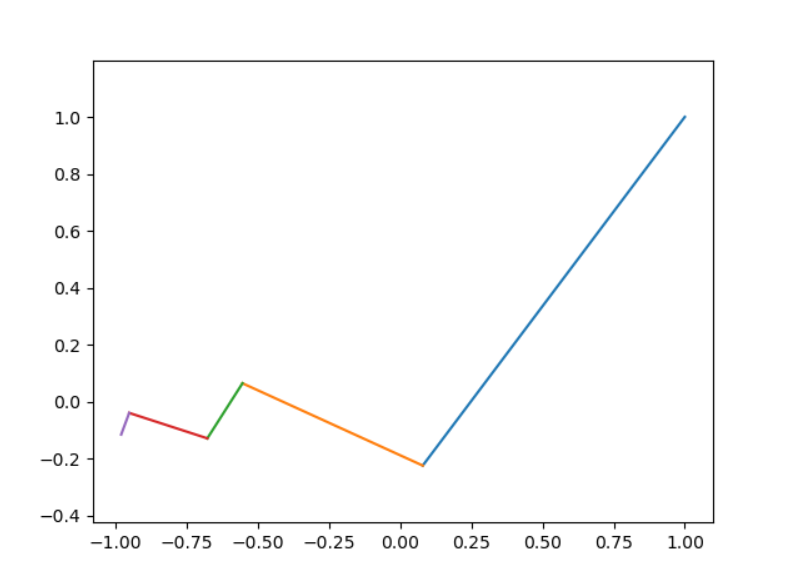
\includegraphics[width=0.5\textwidth]{proof1}
    \caption{$\varepsilon=0.1$}
    \label{fig:proof1}
\end{figure}
\newpage
\begin{figure}[!htb]
    \centering
    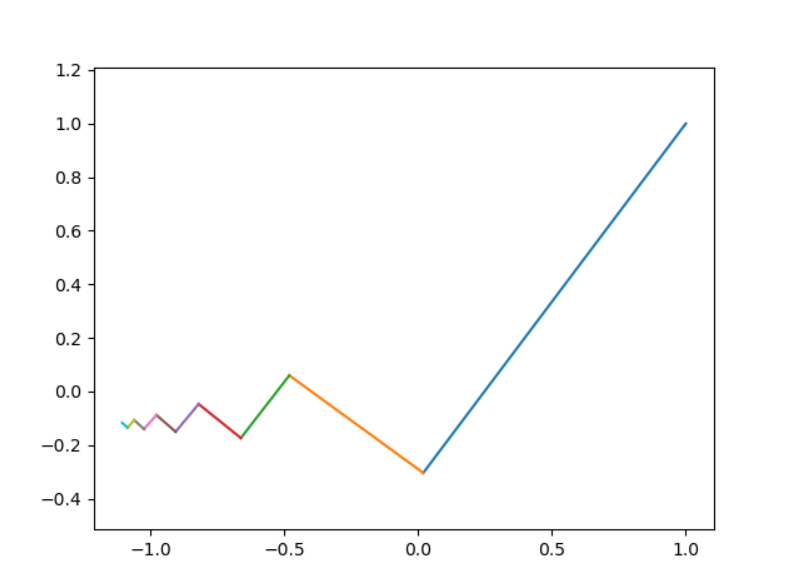
\includegraphics[width=0.5\textwidth]{proof2}
    \caption{$\varepsilon=0.01$}
    \label{fig:proof2}
\end{figure}
\begin{figure}[!htb]
    \centering
    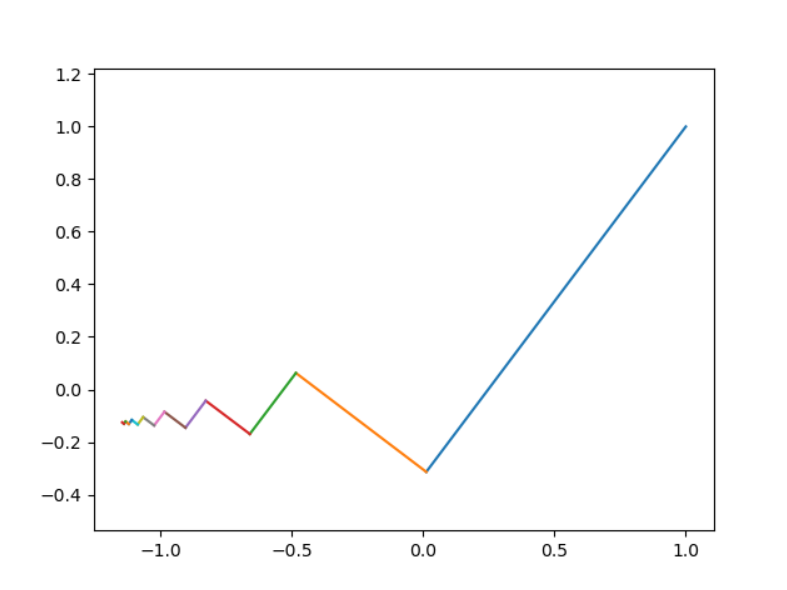
\includegraphics[width=0.5\textwidth]{proof3}
    \caption{$\varepsilon=0.001$}
    \label{fig:proof3}
\end{figure}

Из таблицы и графиков видно, что, чем выше требуемая точность, тем более ``ортогональны `` векторы. Это связано с тем, что при поиске $\alpha$ применяется метод одномерной минимизации с той же заданной точностью, с которой применяется сам градиентный метод.


\section{Обоснование достоверности полученного результата}
Достоверность полученного результата гарантируется теоремами о сходимости, выполнение условий которых проверено в соответствующем разделе отчета.


\end{document}
